
%(BEGIN_QUESTION)
% Copyright 2011, Tony R. Kuphaldt, released under the Creative Commons Attribution License (v 1.0)
% This means you may do almost anything with this work of mine, so long as you give me proper credit

``Off-grid'' electric power systems using solar panels (photovoltaic), wind turbines, and other ambient-energy generators to charge battery banks often enter states where more power is being generated than is needed by loads or to charge the batteries.  It would be a shame to let this unwanted power go to waste, and so these systems are often equipped with {\it dump loads} which may be activated to put the excess power to productive use.  The best ``dump loads'' are those which perform some useful task such as water heating, UV water disinfection, etc.

In this system, a voltage transmitter (ET) senses the DC bus voltage of the power system and reports that to a voltage indicating controller (EIC) with a setpoint of 30 volts.  A current transmitter (IT) senses charging current to the battery bank and reports that to a current indicating controller (IIC) with a setpoint of 28 amps.  A pulse-width modulation (PWM) power controller sends DC power to the dump load at the command of a 4-20 mA signal (the greater the 4-20 mA signal, the higher the duty cycle on the PWM power controller, sending more power to the dump load):

$$\includegraphics[width=15.5cm]{i04599x01.eps}$$

The question is how to arrange these two controllers (EIC and IIC) in some sort of control strategy to prevent over-charging of the battery bank?

\vfil 

\underbar{file i04599}
\eject
%(END_QUESTION)





%(BEGIN_ANSWER)

This is a graded question -- no answers or hints given!

%(END_ANSWER)





%(BEGIN_NOTES)

Batteries may be damaged by excessive charging voltage {\it as well as} excessive charging current, so both controllers need to have a limiting effect: if the voltage is too high, turn on the dump load; if the current is too high, turn on the dump load.  Therefore, the dump load should be controlled by which ever controller sends out the highest signal (i.e. which ever one calls for more power to be diverted away from the batteries).

Since we are dealing with two different -- and possible competing -- criteria for controlling the dump load, we know we must use an {\it override} control strategy in this system.  We must provide a way for either the current controller or the voltage controller to ``take over'' control of the PWM power controller to prevent the battery bank from being over-charged.

\vskip 10pt

Therefore, a reasonable solution would be to have both controllers' outputs feed through a selector function to send a command signal to the PWM unit.  Since the goal here is for either of the controllers to send the PWM unit a greater signal to command more power to be ``dumped,'' we will use a {\it high-select} function for the override selector:

$$\includegraphics[width=15.5cm]{i04599x02.eps}$$

Although not requested in the question, you can see that the directions of action for each controller are shown in this answer.  Determining the proper directions of action for controllers in an override system is critically important for the proper operation of that system.

Since we know the selector function will be a high-select, the only way a controller will become selected and save the battery bank from over-charging is if its output signal is greater than the other controller's.  Since we know the conditions we're trying to avoid with this control system are (1) too much voltage, and/or (2) too much current, we know that the conditions necessitating controller intervention will be that of {\it high} PV values.  If a high PV value is supposed to generate a high controller output to prevent over-charging, those controllers must both be direct-acting.

%INDEX4 Control, strategies: override control

%(END_NOTES)

